% =============================================================================
%  Avance de los tres documentos de la Maestría en Inteligencia Artificial
%  Presentación de avance ante la Subcomisión
%
%  Compilar con:
%     pdflatex avance_maestria_ia.tex   (dos o tres veces)
%  o bien:
%     make
% =============================================================================

\documentclass[10pt,aspectratio=169]{beamer}

% --- Paquetes ----------------------------------------------------------------
\usepackage[utf8]{inputenc}
\usepackage[T1]{fontenc}
\usepackage[spanish]{babel}
\usepackage{lmodern}
\usepackage{microtype}
\usepackage{booktabs}
\usepackage{array}
\usepackage{tikz}
\usetikzlibrary{calc,arrows.meta,positioning,shapes.geometric,backgrounds,fit}

% --- Tema y colores ----------------------------------------------------------
\usetheme{Madrid}
\usecolortheme{seahorse}
\definecolor{accentblue}{RGB}{31,73,125}
\definecolor{accentgreen}{RGB}{46,125,50}
\definecolor{accentorange}{RGB}{214,121,32}
\definecolor{accentred}{RGB}{178,45,45}
\definecolor{lightgray}{RGB}{245,246,248}

\setbeamercolor{frametitle}{bg=accentblue,fg=white}
\setbeamercolor{title}{fg=accentblue}
\setbeamercolor{block title}{bg=accentblue!15,fg=accentblue}
\setbeamercolor{block title alerted}{bg=accentgreen!18,fg=accentgreen}
\setbeamercolor{block title example}{bg=accentorange!18,fg=accentorange}
\setbeamertemplate{navigation symbols}{}
\setbeamertemplate{footline}[frame number]

% --- Datos -------------------------------------------------------------------
\title{Avance de los tres documentos\\
       de la Maestría en Inteligencia Artificial}
\subtitle{Plan de estudio \textbullet\ Plan de factibilidad \textbullet\ Diagnóstico}
\institute{Universidad Nacional Autónoma de Honduras}
\author{Subcomisión de la Maestría en Inteligencia Artificial}
\date{Octubre de 2026}

% --- Macros ------------------------------------------------------------------
\newcommand{\doc}[1]{\textbf{\textcolor{accentblue}{#1}}}
\newcommand{\estado}[1]{\textcolor{accentgreen}{\textbf{#1}}}
\newcommand{\pendiente}{\textcolor{accentorange}{\textbf{[pendiente]}}}

% Cajas de estado (ancho opcional: \textwidth por defecto, \linewidth dentro de tablas)
\newcommand{\estadoverde}[2][\textwidth]{%
  \begin{beamercolorbox}[wd=#1,sep=0.6ex,rounded=true]{item}
    \textcolor{accentgreen}{$\checkmark$\ \textbf{#2}}
  \end{beamercolorbox}}
\newcommand{\estadoambar}[2][\textwidth]{%
  \begin{beamercolorbox}[wd=#1,sep=0.6ex,rounded=true]{item}
    \textcolor{accentorange}{$\bullet$\ \textbf{#2}}
  \end{beamercolorbox}}

% =============================================================================
\begin{document}

% ---------------------------------------------------------------- Portada ----
{\setbeamertemplate{frametitle}{}
\begin{frame}[plain]
  \titlepage
  \vspace{1.2cm}
  \begin{center}
    \begin{beamercolorbox}[wd=0.86\textwidth,sep=1.0ex,rounded=true]{title}
      \centering\small
      \textbf{Facultad de Ciencias}\\[0.2ex]
      {\footnotesize Escuela de Matemáticas --- UNAH}
    \end{beamercolorbox}
  \end{center}
\end{frame}}

% ------------------------------------------------------------- Agenda --------
\begin{frame}{Contenido}
  \tableofcontents
\end{frame}

% =========================================================== SECCIÓN 1 =====
\section*{Punto de partida: los tres documentos}

\begin{frame}{Los tres documentos y su propósito}
  \small
  La UNAH requiere tres documentos que
  sustentan academicamente las propuestas de programas de estudio. Cada uno responde una pregunta distinta
  y juntos conforman el expediente de propuesta.

  \medskip
  \begin{columns}[t]
    \begin{column}{0.31\textwidth}
      \begin{block}{\footnotesize\doc{Plan de estudio}}
        \footnotesize
        \textbf{¿Qué se enseña?}\\
        Estructura curricular: ejes, cursos, créditos, horas de
        estudio supervisado e independiente.
      \end{block}
    \end{column}
    \begin{column}{0.31\textwidth}
      \begin{block}{\footnotesize\doc{Plan de factibilidad}}
        \footnotesize
        \textbf{¿Se puede hacer?}\\
        Condiciones de implementación: planta docente disponible,
        recursos, infraestructura y prerrequisitos institucionales.
      \end{block}
    \end{column}
    \begin{column}{0.31\textwidth}
      \begin{block}{\footnotesize\doc{Diagnóstico}}
        \footnotesize
        \textbf{¿Por qué es necesario?}\\
        Situación actual de la formación en IA en el país y la región,
        vacíos identificados y pertinencia del programa.
      \end{block}
    \end{column}
  \end{columns}

  \medskip
  \begin{alertblock}{Subcomisión de Diseño}
    \footnotesize
    La Subcomisión de diseño se encarga de la redacción de estos documentos, con la colaboración de la DSEP y consultores etc.
  \end{alertblock}
\end{frame}

\begin{frame}{Estado de avance a la fecha}
  \small
  \begin{center}
      \begin{tabular}{@{}
        >{\raggedright\arraybackslash}p{3.2cm}
        >{\raggedright\arraybackslash}p{2.7cm}
        >{\raggedright\arraybackslash}p{2.8cm}
        >{\raggedright\arraybackslash}p{\dimexpr\textwidth-8.7cm-6\tabcolsep\relax}@{}}
    \toprule
    \textbf{Documento} & \textbf{Estado} & \textbf{Correcciones} &
    \textbf{Acción pendiente} \\
    \midrule
    \doc{Plan de estudio}
    & \textcolor{accentorange}{En Consolidación}
      & \estado{Últimas aplicadas}
      & Unificar \emph{todas} las correcciones en un solo documento \\
    \doc{Plan de factibilidad}
      & \estadoverde[\linewidth]{Completo}
      & \estado{Aplicadas}
      & Listo para última revisión \\
    \doc{Diagnóstico}
      & \estadoverde[\linewidth]{Completo}
      & \estado{Aplicadas}
      & Listo para última revisión \\
    \bottomrule
  \end{tabular}
  \end{center}

  \medskip
  \begin{block}{?`Qué es \emph{Consolidación}}
    \footnotesize
    Para agilizar el proceso de revisión, decidimos trabajar en paralelo. \\
    Ahora debemos unir todas las correcciones para presentar un documento final para su aprobación final.\\
    El documento ya tiene \estado{333 páginas}, no queremos agregar más contenido.\\
    \textbf{Es posible que los documentos de factibilidad y diagnóstico presenten nuevas correcciones}.
  \end{block}
\end{frame}

% =========================================================== SECCIÓN 2 =====
\section{Plan de estudio}

%%%%  FRAME  %%%%
\begin{frame}
    \frametitle{Plan de estudio: ejemplos de correcciones}
    El documento tiene \estado{164 observaciones} es su etapa final.\\[0.5em]
    La mayoría de las correcciones son muy sencillas:
    \begin{figure}
        \centering
    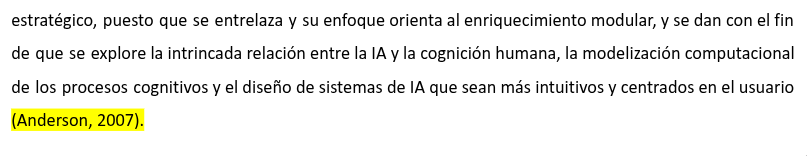
\includegraphics[width=0.8\textwidth]{images/correccion-facil.png}
    \end{figure}
    \pause
    Pero algunas son más delicadas:
    \begin{figure}
        \centering
    
\includegraphics[width=0.5\textwidth]{images/correccion-dificil.png}
    \end{figure}

\end{frame}
%\begin{frame}{Plan de estudio: en qué consiste la consolidación}
%  \small
%  El Plan de estudio es el documento que más cambios ha recibido. Cada
%  observación de la Subcomisión se atendió de forma aislada, lo que dejó el
%  texto \emph{correcto en contenido pero disperso en la forma}.
%
%  \medskip
%  \begin{columns}[t]
%    \begin{column}{0.46\textwidth}
%      \begin{block}{Situación actual}
%        \footnotesize
%        \begin{itemize}
%          \item Correcciones ya incorporadas: \estado{completas}
%          \item Redactos paralelos o duplicados por observación
%          \item Orden de secciones que ya no refleja el flujo aprobado
%          \item Formato heterogéneo entre secciones
%        \end{itemize}
%      \end{block}
%    \end{column}
%    \begin{column}{0.46\textwidth}
%      \begin{block}{Trabajo pendiente}
%        \footnotesize
%        \begin{itemize}
%          \item Versión única consolidada de todo el documento
%          \item Verificación de \emph{coherencia horizontal}
%          \item Cotejo final contra la factibilidad y el diagnóstico
%          \item Cumplimiento de formato institucional
%        \end{itemize}
%      \end{block}
%    \end{column}
%  \end{columns}
%
%  \vfill
%  \begin{alertblock}{Riesgo a evitar}
%    \footnotesize
%    Consolidar no debe introducir \emph{nuevos} cambios de fondo. La
%    edición es de forma; el contenido ya fue revisado por la Subcomisión.
%  \end{alertblock}
%\end{frame}

%\begin{frame}{Plan de estudio: alcance de las últimas correcciones}
%  \small
%  \begin{columns}[t]
%    \begin{column}{0.5\textwidth}
%      \begin{block}{Correcciones incorporadas}
%        \footnotesize
%        \begin{itemize}
%          \item \pendiente\ --- % dejar vacío o completar
%          \item \pendiente
%          \item \pendiente
%        \end{itemize}
%      \end{block}
%    \end{column}
%    \begin{column}{0.5\textwidth}
%      \begin{block}{Pendiente de aplicar}
%        \footnotesize
%        \begin{itemize}
%          \item \pendiente
%          \item \pendiente
%          \item \pendiente
%        \end{itemize}
%      \end{block}
%    \end{column}
%  \end{columns}
%
%  \medskip
%  \begin{block}{Verificación de la consolidación}
%    \footnotesize
%    \begin{enumerate}
%      \item Un solo archivo, sin versiones divergentes circulando.
%      \item Cada corrección de la Subcomisión con su trazabilidad.
%      \item Checklist de formato institucional firmado por el responsable.
%      \item Circular junto con los otros dos documentos a revisión final.
%    \end{enumerate}
%  \end{block}
%\end{frame}

% =========================================================== SECCIÓN 3 =====
\section{Plan de factibilidad}

%\begin{frame}{Plan de factibilidad: listo para última revisión}
%  \small
%  Responde a la pregunta central de cualquier propuesta de maestría:
%  \emph{¿existen las condiciones reales para operar el programa?}
%
%  \medskip
%  \begin{columns}[t]
%    \begin{column}{0.48\textwidth}
%      \begin{block}{Contenido verificado}
%        \footnotesize
%        \begin{itemize}
%          \item \pendiente\ % planta docente disponible
%          \item \pendiente
%          \item \pendiente
%          \item \pendiente
%        \end{itemize}
%      \end{block}
%    \end{column}
%    \begin{column}{0.48\textwidth}
%      \begin{block}{Qué revisaremos}
%        \footnotesize
%        \begin{itemize}
%          \item Consistencia con la carga académica del plan de estudio
%          \item Factores de conversión: supuesto frente a dato
%          \item Actualidad de los datos oficiales
%          \item Formato institucional
%        \end{itemize}
%      \end{block}
%    \end{column}
%  \end{columns}
%
%  \medskip
%  \estadoverde{Documento completo --- listo para última revisión}
%\end{frame}

% =========================================================== SECCIÓN 4 =====
\section{Diagnóstico}

%\begin{frame}{Diagnóstico: listo para última revisión}
%  \small
%  Es el documento que fundamenta la \emph{necesidad} del programa. Debe
%  sostener, con evidencia, que existe un vacío de formación en IA y que la
%  Maestría es la respuesta pertinente.
%
%  \medskip
%  \begin{columns}[t]
%    \begin{column}{0.48\textwidth}
%      \begin{block}{Contenido verificado}
%        \footnotesize
%        \begin{itemize}
%          \item \pendiente\ % situación actual y vacíos
%          \item \pendiente
%          \item \pendiente
%          \item \pendiente
%        \end{itemize}
%      \end{block}
%    \end{column}
%    \begin{column}{0.48\textwidth}
%      \begin{block}{Qué revisaremos}
%        \footnotesize
%        \begin{itemize}
%          \item Solidez de las fuentes citadas
%          \item Actualidad de las cifras
%          \item Coherencia con el perfil de egreso del plan de estudio
%          \item Que la necesidad quede explicitada sin ambigüedad
%        \end{itemize}
%      \end{block}
%    \end{column}
%  \end{columns}
%
%  \medskip
%  \estadoverde{Documento completo --- listo para última revisión}
%\end{frame}

% =========================================================== SECCIÓN 5 =====
\section*{Cierre}

\begin{frame}{Compromisos y próximos pasos}
    \framesubtitle{Como equipo, la Subcomisión se encuentra comprometida a finalizar el proceso.}
  \small
  \begin{columns}[t]
    \begin{column}{0.48\textwidth}
        \begin{block}{Siguientes pasos}
        \footnotesize
             \estadoverde{Consolidación}
            \estadoambar{Presentacion a la DSEP}
            \estadoambar{Presentación a la Facultad}
            \estadoambar{Aprobación del Consejo}
      \end{block}
    \end{column}
    \begin{column}{0.48\textwidth}
      \begin{block}{Plazos}
        \footnotesize
        \begin{tabular}{@{}ll@{}}
          \toprule
          Hito & Fecha \\
          \midrule
          Consolidación & 17/oct \\
          Reunion DSEP & finales de oct \\
          Facultad & 6/nov\\
          Consejo & ????\\
          \bottomrule
        \end{tabular}
      \end{block}
    \end{column}
  \end{columns}

  \vfill
  \begin{alertblock}{Siguientes pasos}
    \footnotesize
    \begin{enumerate}
        \item Finalizar el proceso de consolidación.
            
      \item Acordar la fecha de corte para la versión consolidada del
          Plan de estudio con la DSEP.
      \item Indicar si se requiere una sesión conjunta de los tres
            documentos antes de la siguiente etapa.
    \end{enumerate}
  \end{alertblock}
\end{frame}

\begin{frame}{!`Gracias!}
  \vspace{0.8cm}
  \centering
  {\Large\doc{Plan de estudio}} \textcolor{gray}{\textbullet}
  {\Large\doc{Plan de factibilidad}} \textcolor{gray}{\textbullet}
  {\Large\doc{Diagnóstico}}


  \vfill
  {\footnotesize\color{gray} Gracias por su atención.}
\end{frame}

\end{document}
